\documentclass[pra,aps,superscriptaddress,reprint]{revtex4-2}
\usepackage{amsmath,amssymb,graphicx}
\usepackage{xeCJK}
\setCJKmainfont{AR PL UMing CN}
\setCJKsansfont{AR PL UKai CN}
\setCJKmonofont{AR PL UKai CN}
\usepackage[colorlinks=true,linkcolor=blue,citecolor=blue,urlcolor=blue]{hyperref}

\begin{document}

% TODO(authors): 替换为真实姓名、单位、邮箱。
\title{广义 Su-Schrieffer-Heeger 链的变分制备与反射拓扑读出：超导硬件实验}

% TODO(authors): 作者顺序已按“邱雪一作、余金龙通讯”排；通讯邮箱待补。
\author{邱雪}
\affiliation{海南大学，中国}
\author{余金龙\thanks{通讯作者。}}
\affiliation{海南大学，中国}
% TODO(邮箱): 在余金龙的 \author 行加 \email{真实邮箱}。

\date{\today}

\begin{abstract}
我们报道一套变分量子计算流程：在云端超导处理器上制备广义
Su-Schrieffer-Heeger 链的基态，并读出其反射对称拓扑性质。反射不变量
$Z_R$ 由基态投影算符构造，数值上给出 $(s,\delta)$ 相图；对称性约束
哈密顿量打开基态简并，每个相区配一个可直接制备的初态；变分绝热路径
用二次 B\'ezier 曲线参数化并做三层优化，硬件实验改用浅层环形电路与
直线轨迹。读出误差缓解、门误差零噪声外推、以及以精确已知的单态为参
考的参考态零噪声外推，使云端硬件能量达到与精确值百分之几的符合。
硬件上 $Z_R$ 的拓扑读出已形成完整协议，部分最终数据点以占位形式给出。
\end{abstract}

\maketitle

\section{引言}
\label{sec:intro}

一维自旋系统的拓扑相以 Su-Schrieffer-Heeger (SSH)
模型为代表~\cite{Su1979,Su1980}，一直是量子模拟的核心检验场：其物理由
Zak 相位等量子化不变量控制~\cite{Zak1989}，相互作用体系则由纠缠谱简
并~\cite{Pollmann2010} 与可测量的多体拓扑不变量刻画~\cite{Elben2020}。
另一方面，含噪声中等规模量子
(NISQ) 处理器~\cite{Preskill2018} 可以变分方式制备关联试探态
~\cite{Peruzzo2014,Kandala2019,Bharti2022}，前提是算法选择尊重真实硬件
严苛的深度与噪声预算，并系统使用误差缓解技术
~\cite{Temme2017,Li2017,Cai2023}。

本工作把这两条线连起来。目标是一条完整、可在硬件上执行的流程：
(i) 用反射不变量 $Z_R$ 给广义 SSH 链基态做拓扑分类；(ii) 用浅层变分
电路制备对应基态；(iii) 在器件上测出拓扑性质。模型研究、对称性分析
与变分设计已完成；云端硬件能量测量（含误差缓解）部分完成；硬件上
$Z_R$ 的最终读出已固定为明确协议，数据点以占位形式留空。

全文安排如下。第~\ref{sec:model} 节定义模型与不变量。
第~\ref{sec:symmetry} 节给出对称性约束与各相区初态。
第~\ref{sec:variational} 节描述变分 ansatz 与路径参数化（含硬件适配
版本）。第~\ref{sec:measure} 节介绍测量工具箱。
第~\ref{sec:mitigation} 节记录读出缓解、零噪声外推 (ZNE) 与参考态
ZNE (rZNE)，复现 Ref.~\cite{Yu2023} 的协议。
第~\ref{sec:results} 节给出数值与硬件结果，
第~\ref{sec:outlook} 节总结展望。

\section{模型与反射不变量}
\label{sec:model}

考虑 $N$ 比特广义 SSH 哈密顿量，交错 $XX+ZZ$ 耦合，
\begin{equation}
\begin{aligned}
H ={}& (1-s) \sum_{i\,\mathrm{odd}} (X_i X_{i+1} + \delta Z_i Z_{i+1}) \\
&+ s \sum_{j\,\mathrm{even}} (X_j X_{j+1} + \delta Z_j Z_{j+1}),
\end{aligned}
\label{eq:H}
\end{equation}
其中 $s\in[0,1]$ 调二聚化强度，$\delta\in[0,1]$ 为 $ZZ$ 各向异性。
总比特数须为 4 的倍数（最少 8），该限制决定初态旋转方式与基态对称
性 sector，详见第~\ref{sec:symmetry} 节。

空间反射对称性由下式量化，
\begin{equation}
Z_R = \frac{\mathrm{tr}(\rho S)}
  {\sqrt{(\mathrm{tr}(\rho_1^2) + \mathrm{tr}(\rho_2^2))/2}},
  \quad
  S = \bigotimes_{i=1}^{N/2} \mathrm{SWAP}_{i,\,N-i+1},
  \label{eq:ZR}
\end{equation}
其中 $\rho$ 为基态投影算符，$\rho_{1,2}$ 为反射 bipartition 的约化态。
下文数值中 $Z_R$ 在三个相区分别取值 $+1$、$-1$、$0$，符号跳变即拓扑
相边界。

\section{对称性约束与初态制备}
\label{sec:symmetry}

绝热制备的常见困难是基态简并：高对称点处多个态竞争，任意叠加在演
化中会漏出目标对称性 sector。我们加入对易观测量打开简并。取
\begin{equation}
U_x = \bigotimes_{i=1}^N X_i, \qquad
U_z = \bigotimes_{i=1}^N Z_i,
\label{eq:UxUz}
\end{equation}
当 $N$ 为 4 的倍数时 $[U_{x,z},H]=0$ 且 $[U_x,U_z]=0$，构造
$P=U_x+2U_z$（本征值 $3,-1,1,-3$），定义约束哈密顿量
\begin{equation}
H_c = H - \epsilon\,P, \qquad \epsilon = 0.05.
\label{eq:Hc}
\end{equation}
惩罚系数 $\epsilon$ 特意取小，避免同对称性激发态被压到目标基态之下；
对称基态能量平移 $-3\epsilon$，波函数从而 $Z_R$ 不变。

每个相区都有可直接制备的初态。$s=0$（$Z_R=+1$ 区）与 $s=1$
（$Z_R=-1$ 区，差边界条件）处哈密顿量是键上对易项之和，基态即最低
能量 Bell 对直积 $(|01\rangle-|10\rangle)^{\otimes N/2}$，一层 $X$、
$H$、CNOT 门即可制备。$Z_R=0$ 区从 $\delta=0$ 出发，此时所有 $XX$ 项
对易；在二重简并流形中对角化 $U_z$，选出
$(|\phi^+\rangle+|\phi^-\rangle)/\sqrt{2}$，
$|\phi^{\pm}\rangle=|\pm\mp\pm\cdots\rangle$，即 $X$ 表象 GHZ 态。边缘
比特由整体约束 $U_x=U_z=1$ 继承固定边界条件。

\section{变分 ansatz 与路径参数化}
\label{sec:variational}

变分方案为三个相区各取一个代表初态
（$p_{\mathrm{idx}}\in\{1,0,-1\}$），沿参数化路径演化并做变分优化，
在每个目标点保留代价最小的分支。代价函数为约束能量加对称性惩罚；
$Z_R$ 距离与演化时间惩罚为可选扩展，留待以后工作。

绝热路径参数化为二次 B\'ezier 曲线，控制点用
$(u_s,u_\delta)\in[0,1]$ 线性换元，绝热态制备的思路见
Ref.~\cite{Albash2018}。优化分三层：外层扫 Trotter 阶数与步数，中层
扫三个初态分支，内层优化连续参数（$v_0$、$u_s$、$u_\delta$、
$\Delta t_n$、$d_n$）。电路用 Pauli 演化门构造，演化路径与步长手动
绑定，门基于开源电路工具包~\cite{Qiskit2023}，并经人工核对转译后仍
保持 even 层优先的门序结构。

硬件经验重塑了 ansatz。云端处理器上噪声使能量系统性偏高，电路越深
偏差越大，连初态保真度都不理想。硬件适配版本于是接受“只能跑极浅电
路”的现实：环形拓扑、直线轨迹（路径与 $\Delta t$ 解耦）、参数远离定
义域边界，目标从“验证方案”改为“硬件最低能量”。Trotter 分层的
even/odd 键 ansatz，
\begin{equation}
|\psi_{\mathrm{ansatz}}(\{\theta\})\rangle
  = \prod_{l=1}^{N_L} U^{(l)}_{\mathrm{even}} U^{(l)}_{\mathrm{odd}}
    |\psi_{\mathrm{singlets}}\rangle,
\label{eq:ansatz}
\end{equation}
每键作用
$\exp(-i\theta_x XX-i\theta_y YY-i\theta_z ZZ)$，且 even 层先作用，
连接了两代设计：它正是第~\ref{sec:mitigation} 节误差缓解复现所用的
形式。

\section{测量工具箱}
\label{sec:measure}

期望值经由自研测量栈的两条互补路径获得。旋转基估计器对逐比特对易
Pauli 项分组，加单比特旋转门后逐组提交硬件任务，由返回直方图重建
Pauli 期望；本地模拟路径则直接调用标准估计器原语。随机测量模块在模
拟与硬件后端实现经典影子风格协议~\cite{Huang2020,Elben2019}，是用以
直接在硬件上估计式~\eqref{eq:ZR} 所需非局域关联函数的既定路线，
精神与 Ref.~\cite{Elben2020} 一致。所有硬件访问经由厂商云接口；本文
任何协议都不需要额外量子资源（辅助比特或编码比特）。

\section{误差缓解}
\label{sec:mitigation}

我们复现并应用 Ref.~\cite{Yu2023} 面向云端超导硬件的三段缓解协议：
(i) 读出误差缓解~\cite{Bravyi2021,Berg2022}，(ii) 门误差 ZNE，
(iii) 参考态 ZNE。读出缓解为每根键标定 $4\times4$ 概率混淆矩阵 $M$
（$\vec P_{\mathrm{measured}}=M\vec P_{\mathrm{ideal}}$，在理想分布非
负约束下反解）；偶/奇键并行标定，开销与系统尺寸无关。Bell 基测量缓
解同理：设 $U$ 为 Bell 态制备电路，则 Bell 基测量等于固定变换
$U^\dagger$ 后接计算基测量；四个标定电路形如
$U^\dagger P U|0\cdots0\rangle$（$P\in\{I,X,Z,XZ\}$），测量端固定、
只换输入端单比特 Pauli 门。

门误差 ZNE 制备
$|\psi_n\rangle=U(U^\dagger U)^n|0\cdots0\rangle$，对
$O_n=\langle\psi_n|\hat O|\psi_n\rangle$ 按 $m=2n+1\to0$ 做指数拟合
$ae^{-bm}+c$ 外推零噪声极限；数据驱动初值
$p_0=[y_0-y_{-1},\,0.3,\,y_{-1}]$ 不可或缺，默认种子会落入梯度消失的
平凡解。方法论亮点 rZNE 用 ansatz 族内参考态——变分参数全零的 Bell
对直积态 $|\psi_{\mathrm{singlets}}\rangle$，其能量精确已知，
$E_{\mathrm{Bell}}=-(2+\Delta)N/2$ 且与插值参数 $s$ 无关。两条硬件
经验一并记录以便复现：厂商后编译会静默删除近零角度门，以下边界
$5.1\times10^{-4}$ 对冲；噪声放缩点数在一代处理器上 $n_m=3$--$4$，
另一代上 $n_m=2$--$3$。变分任务的 ZNE 实践另见
Refs.~\cite{Uvarov2024,Kurita2023,GiurgicaTiron2020}。

\section{结果}
\label{sec:results}

\subsection{数值相图与相边界}
\label{sec:phase}

$N=8$ 时在 $(s,\delta)\in[0,1]^2$ 取 $100\times100$ 格点求基态，对边
缘 4 比特求偏迹后计算式~\eqref{eq:ZR}。图~\ref{fig:phase} 显示三个截
然分开的相区：$s=0$ 一侧 $Z_R\approx+1$，$s=1$ 一侧
$Z_R\approx-1$，另有一 $Z_R\approx0$ 楔形向 $\delta\to0$ 张开。

\begin{figure}[tbp]
\centering
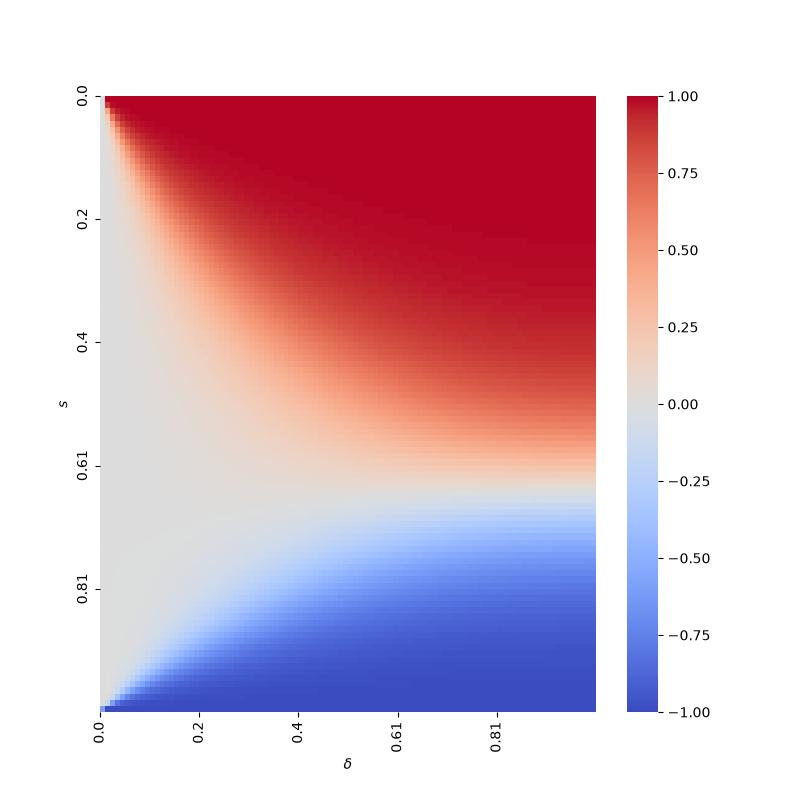
\includegraphics[width=\columnwidth]{figs/fig_phase_N8.jpg}
\caption{$N=8$ 的 $Z_R$ 热力图：精确对角化并对 4 个边缘比特求偏迹。
$Z_R\approx+1$、$-1$、$0$ 三个相区沿清晰边界相接。
\label{fig:phase}}
\end{figure}

相边界由 $Z_R=0$ 穿零点定义：先固定 $\delta=1$ 提取临界 $s_p$，再在
固定 $s$ 切线取 $\delta_p$。图~\ref{fig:boundary} 显示 $s_p$ 随尺寸
漂移（$N=8$ 时 $0.640$，$N=12$ 时 $0.622$，$N=16$ 时 $0.612$），而
$\delta_p$ 切线基本不随 $N$ 变化，表明边界在 $\delta$ 方向收敛快于
$s$ 方向。

\begin{figure*}[tbp]
\centering
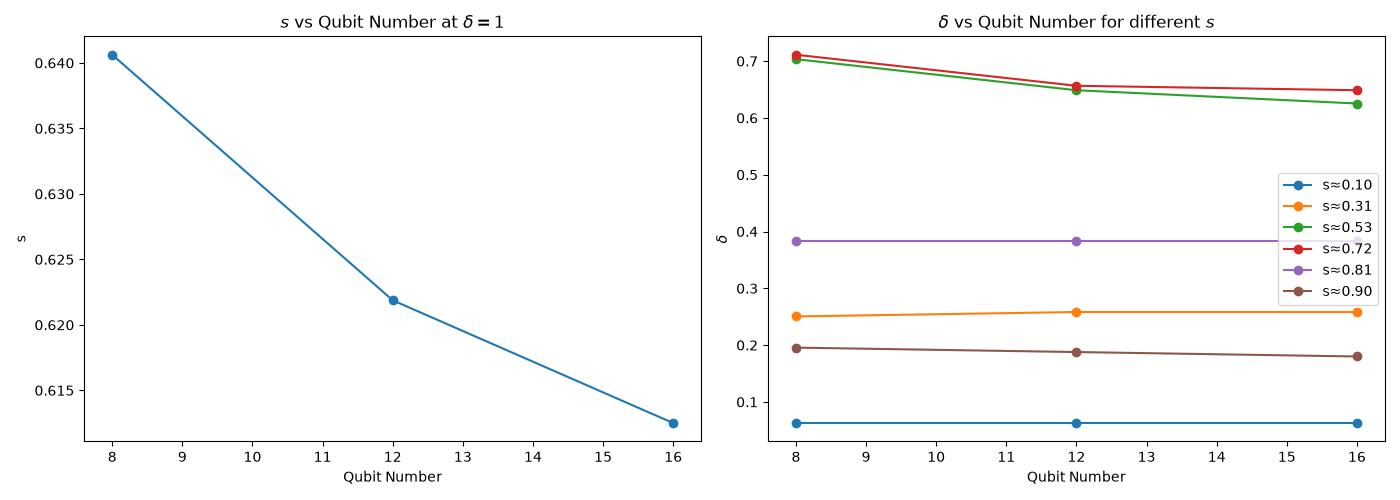
\includegraphics[width=0.9\textwidth]{figs/fig_phase_boundary.jpg}
\caption{$Z_R=0$ 边界的有限尺寸标度。左：$\delta=1$ 处临界 $s_p$ 随比
特数变化。右：固定 $s$ 切线的临界 $\delta_p$ 随比特数变化；在分辨范
围内基本平坦。
\label{fig:boundary}}
\end{figure*}

\subsection{约束验证}
\label{sec:constraint}

在式~\eqref{eq:Hc} 的 $H_c$ 下重扫 $Z_R$ 相图不变，而低能谱分列：对
称基态与其简并伙伴分开。图~\ref{fig:constraint} 并排比较 $N=8$ 无约
束与有约束热力图；$s$、$\delta$ 扫描的能谱（最低 $k=4$、$k=8$ 能级，
$N=8$、$N=12$）随数值数据集存档。

\begin{figure}[tbp]
\centering
\begin{minipage}{0.49\columnwidth}
\centering
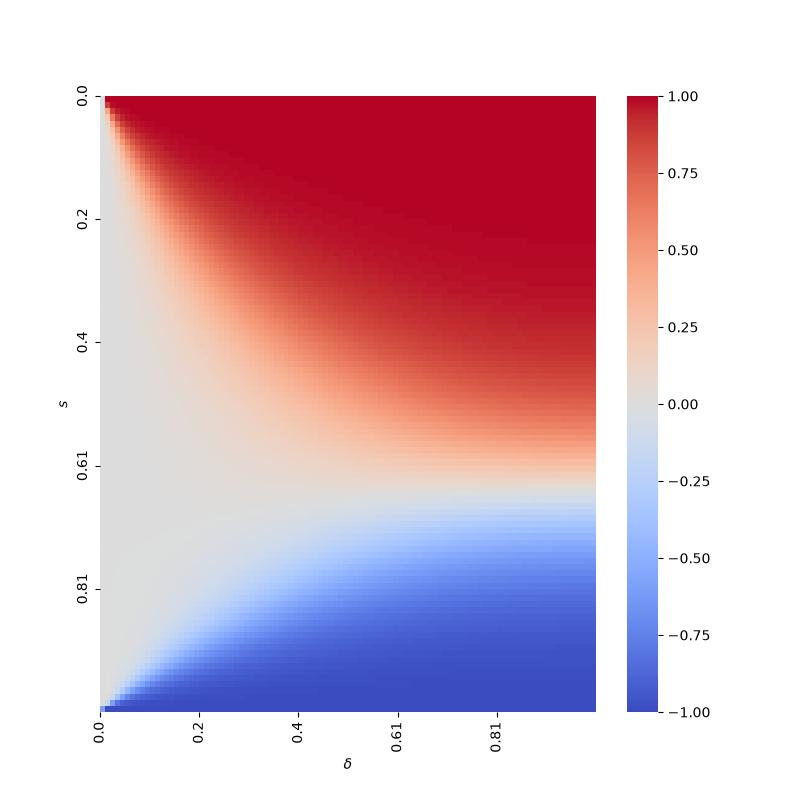
\includegraphics[width=\textwidth]{figs/fig_phase_N8.jpg}
\\(a) 无约束
\end{minipage}
\hfill
\begin{minipage}{0.49\columnwidth}
\centering
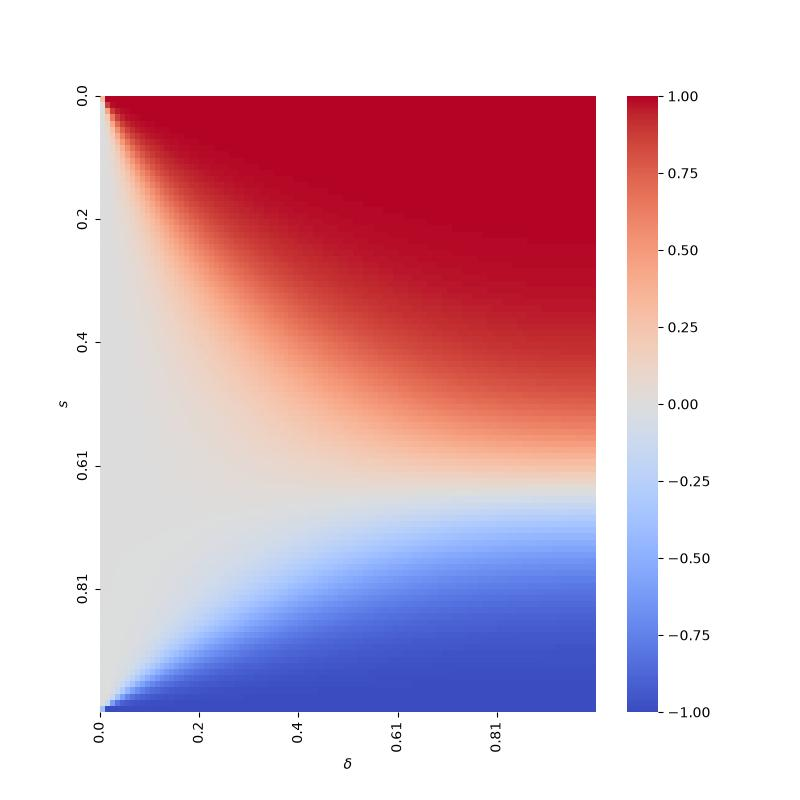
\includegraphics[width=\textwidth]{figs/fig_phase_constrained_N8.jpg}
\\(b) 有约束
\end{minipage}
\caption{$N=8$ 的 $Z_R$ 热力图：(a) 无式~\eqref{eq:Hc} 对称性惩罚，
(b) 有惩罚。基态波函数从而 $Z_R$ 不变，只有能谱分列。
\label{fig:constraint}}
\end{figure}

\subsection{硬件能量：ZNE 与 rZNE}
\label{sec:hardware}

图~\ref{fig:exemplary} 为云端处理器 $s=1$ 处代表性拟合：外推能量自
含噪原始值移向精确值；以 $E_{\mathrm{Bell}}=-12.0$ 为参考的 rZNE 在
Bell 电路上给出 $-12.000$，在完整 ansatz 电路上给出 $-14.278$（精确
值 $-13.500$），而普通 ZNE 为 $-9.015$。沿 $s\in[0,1]$ 扫描，rZNE 基
态能量点聚在精确基态曲线周围，纯 ZNE 点整体偏高
（图~\ref{fig:specscan}）。

\begin{figure}[tbp]
\centering
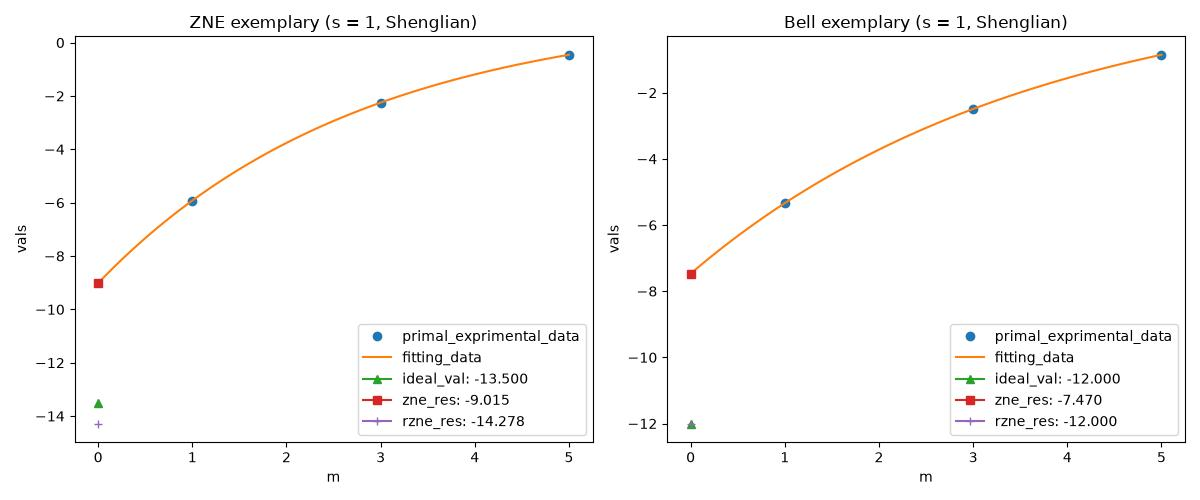
\includegraphics[width=0.8\columnwidth,trim={0 0 510 0},clip]{figs/fig_rzne_exemplary.jpg}
(a) 完整 ansatz 电路
\\[\smallskipamount]
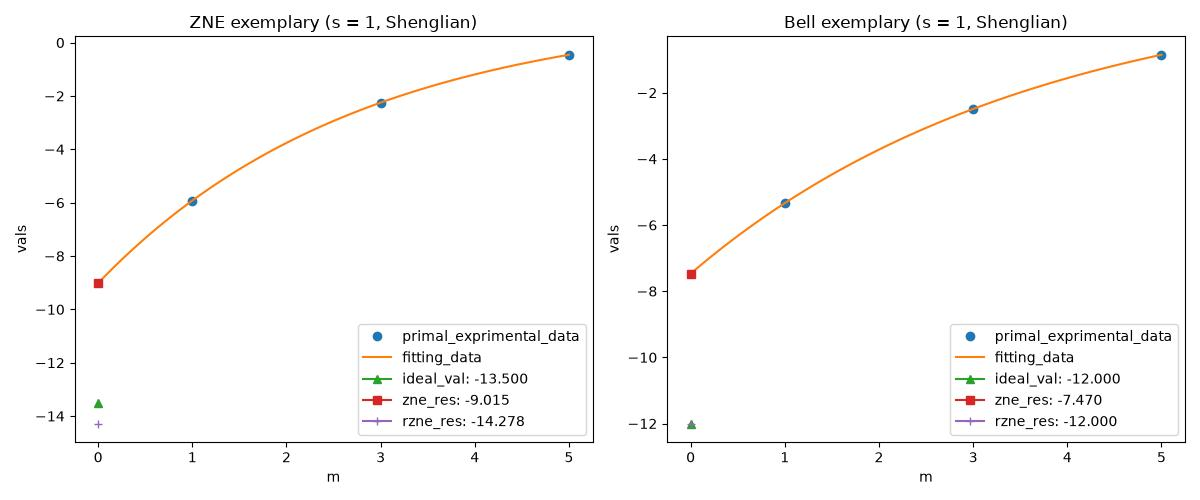
\includegraphics[width=0.8\columnwidth,trim={790 0 0 0},clip]{figs/fig_rzne_exemplary.jpg}
(b) Bell 参考电路
\caption{噪声标度 $m=2n+1$ 下的指数拟合 $ae^{-bm}+c$ 代表例（$s=1$）。
(a) 完整 ansatz 电路（精确值 $-13.500$；ZNE $-9.015$；rZNE
$-14.278$）。(b) Bell 参考电路（精确值 $-12.000$；ZNE $-7.470$；
rZNE $-12.000$）。
\label{fig:exemplary}}
\end{figure}

\begin{figure}[tbp]
\centering
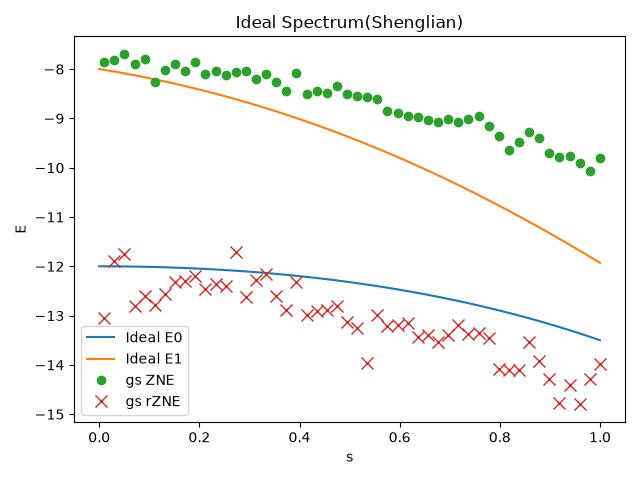
\includegraphics[width=0.85\columnwidth]{figs/fig_rzne_spectrum.jpg}
\caption{基态能量随 $s$ 变化：精确 $E_0$（蓝）、$E_1$（橙）曲线，
硬件 ZNE（绿点）与 rZNE（红叉）。rZNE 点在整个扫描区间聚在精确基态
曲线周围。
\label{fig:specscan}}
\end{figure}

\subsection{硬件拓扑读出（协议已定，数据待补）}
\label{sec:readout}

% TODO(data): 填入各 (s,delta) 实测 Z_R 值。
硬件测量 $Z_R$ 走固定协议：制备优化后 ansatz 态，按
第~\ref{sec:mitigation} 节做 Bell 基对测量（含读出缓解），重建反射
算符 $S$ 所需两体关联，结合独立测量的纯度按式~\eqref{eq:ZR} 合成。
图~\ref{fig:readout} 预留版式（固定 $\delta$ 下实测 $Z_R$ 随 $s$ 变
化，叠加数值边界），待数据运行补入。

\begin{figure}[tbp]
\centering
\fbox{\parbox{0.9\columnwidth}{\centering \vspace{0.8cm}
TODO：实测 $Z_R$ 随 $s$ 变化（含误差棒），叠加数值 $Z_R=0$ 边界。
\vspace{0.8cm}}}
\caption{硬件拓扑读出占位图。正式版将给出固定 $\delta$ 下实测 $Z_R$
随 $s$ 变化，误差棒来自随机测量模块的统计分析。
\label{fig:readout}}
\end{figure}

\section{讨论与展望}
\label{sec:outlook}

我们展示了一条端到端的变分流程：从不变量映射、对称性感知的态制备，
到误差缓解后与精确值符合到百分之几的硬件能量。剩下的一步——非局域
不变量 $Z_R$ 的硬件读出——只需执行已记录的协议；分析链（缓解、关联
重建、纯度归一）已经就位。自然的扩展是把硬件规模推到 $N=12$、$N=16$
（数值边界已画好），并把读出移植到随机测量估计器，直接比较采样开销。

\begin{acknowledgments}
感谢所用开源量子软件栈的开发者与维护者。云端硬件机时由厂商学术计划
提供。基金信息待补。
\end{acknowledgments}

\clearpage
\appendix

\section{指数拟合初值}
\label{app:fit}

用 \texttt{scipy.optimize.curve\_fit} 按默认种子 $p_0=[1,1,1]$ 拟合
$ae^{-bm}+c$ 会塌到平凡解：$b$ 增大时指数项消失、梯度消失，$a$、$b$
不可辨识。数据驱动种子 $p_0=[y_0-y_{-1},\,0.3,\,y_{-1}]$（振幅取首尾
差、衰减率取经验值、渐近项取末值）在本文全部硬件数据集上恢复稳定收
敛。

\section{二次 B\'ezier 路径细节}
\label{app:bezier}

绝热路径控制点线性换元为 $(u_s,u_\delta)\in[0,1]$；优化器把步长推到
定义域边缘时对 $\Delta t\in[0,1]$ 加边界保护。每 Trotter 步 even 键层
先于 odd 键层作用，因为单态直积初态恰为 $H_{\mathrm{odd}}$ 本征态，
打头的 odd 层只贡献全局相位。

%apsrev4-2.bst 2019-01-14 (MD) hand-edited version of apsrev4-1.bst
%Control: key (0)
%Control: author (8) initials jnrlst
%Control: editor formatted (1) identically to author
%Control: production of article title (0) allowed
%Control: page (0) single
%Control: year (1) truncated
%Control: production of eprint (0) enabled
\begin{thebibliography}{22}%
\makeatletter
\providecommand \@ifxundefined [1]{%
 \@ifx{#1\undefined}
}%
\providecommand \@ifnum [1]{%
 \ifnum #1\expandafter \@firstoftwo
 \else \expandafter \@secondoftwo
 \fi
}%
\providecommand \@ifx [1]{%
 \ifx #1\expandafter \@firstoftwo
 \else \expandafter \@secondoftwo
 \fi
}%
\providecommand \natexlab [1]{#1}%
\providecommand \enquote  [1]{``#1''}%
\providecommand \bibnamefont  [1]{#1}%
\providecommand \bibfnamefont [1]{#1}%
\providecommand \citenamefont [1]{#1}%
\providecommand \href@noop [0]{\@secondoftwo}%
\providecommand \href [0]{\begingroup \@sanitize@url \@href}%
\providecommand \@href[1]{\@@startlink{#1}\@@href}%
\providecommand \@@href[1]{\endgroup#1\@@endlink}%
\providecommand \@sanitize@url [0]{\catcode `\\12\catcode `\$12\catcode
  `\&12\catcode `\#12\catcode `\^12\catcode `\_12\catcode `\%12\relax}%
\providecommand \@@startlink[1]{}%
\providecommand \@@endlink[0]{}%
\providecommand \url  [0]{\begingroup\@sanitize@url \@url }%
\providecommand \@url [1]{\endgroup\@href {#1}{\urlprefix }}%
\providecommand \urlprefix  [0]{URL }%
\providecommand \Eprint [0]{\href }%
\providecommand \doibase [0]{https://doi.org/}%
\providecommand \selectlanguage [0]{\@gobble}%
\providecommand \bibinfo  [0]{\@secondoftwo}%
\providecommand \bibfield  [0]{\@secondoftwo}%
\providecommand \translation [1]{[#1]}%
\providecommand \BibitemOpen [0]{}%
\providecommand \bibitemStop [0]{}%
\providecommand \bibitemNoStop [0]{.\EOS\space}%
\providecommand \EOS [0]{\spacefactor3000\relax}%
\providecommand \BibitemShut  [1]{\csname bibitem#1\endcsname}%
\let\auto@bib@innerbib\@empty
%</preamble>
\bibitem [{\citenamefont {Su}\ \emph {et~al.}(1979)\citenamefont {Su},
  \citenamefont {Schrieffer},\ and\ \citenamefont {Heeger}}]{Su1979}%
  \BibitemOpen
  \bibfield  {author} {\bibinfo {author} {\bibfnamefont {W.~P.}\ \bibnamefont
  {Su}}, \bibinfo {author} {\bibfnamefont {J.~R.}\ \bibnamefont {Schrieffer}},\
  and\ \bibinfo {author} {\bibfnamefont {A.~J.}\ \bibnamefont {Heeger}},\
  }\bibfield  {title} {\bibinfo {title} {Solitons in polyacetylene},\ }\href
  {https://doi.org/10.1103/PhysRevLett.42.1698} {\bibfield  {journal} {\bibinfo
   {journal} {Phys. Rev. Lett.}\ }\textbf {\bibinfo {volume} {42}},\ \bibinfo
  {pages} {1698} (\bibinfo {year} {1979})}\BibitemShut {NoStop}%
\bibitem [{\citenamefont {Su}\ \emph {et~al.}(1980)\citenamefont {Su},
  \citenamefont {Schrieffer},\ and\ \citenamefont {Heeger}}]{Su1980}%
  \BibitemOpen
  \bibfield  {author} {\bibinfo {author} {\bibfnamefont {W.~P.}\ \bibnamefont
  {Su}}, \bibinfo {author} {\bibfnamefont {J.~R.}\ \bibnamefont {Schrieffer}},\
  and\ \bibinfo {author} {\bibfnamefont {A.~J.}\ \bibnamefont {Heeger}},\
  }\bibfield  {title} {\bibinfo {title} {Soliton excitations in
  polyacetylene},\ }\href {https://doi.org/10.1103/PhysRevB.22.2099} {\bibfield
   {journal} {\bibinfo  {journal} {Phys. Rev. B}\ }\textbf {\bibinfo {volume}
  {22}},\ \bibinfo {pages} {2099} (\bibinfo {year} {1980})}\BibitemShut
  {NoStop}%
\bibitem [{\citenamefont {Zak}(1989)}]{Zak1989}%
  \BibitemOpen
  \bibfield  {author} {\bibinfo {author} {\bibfnamefont {J.}~\bibnamefont
  {Zak}},\ }\bibfield  {title} {\bibinfo {title} {Berry's phase for energy
  bands in solids},\ }\href {https://doi.org/10.1103/PhysRevLett.62.2747}
  {\bibfield  {journal} {\bibinfo  {journal} {Phys. Rev. Lett.}\ }\textbf
  {\bibinfo {volume} {62}},\ \bibinfo {pages} {2747} (\bibinfo {year}
  {1989})}\BibitemShut {NoStop}%
\bibitem [{\citenamefont {Pollmann}\ \emph {et~al.}(2010)\citenamefont
  {Pollmann}, \citenamefont {Turner}, \citenamefont {Berg},\ and\ \citenamefont
  {Oshikawa}}]{Pollmann2010}%
  \BibitemOpen
  \bibfield  {author} {\bibinfo {author} {\bibfnamefont {F.}~\bibnamefont
  {Pollmann}}, \bibinfo {author} {\bibfnamefont {A.~M.}\ \bibnamefont
  {Turner}}, \bibinfo {author} {\bibfnamefont {E.}~\bibnamefont {Berg}},\ and\
  \bibinfo {author} {\bibfnamefont {M.}~\bibnamefont {Oshikawa}},\ }\bibfield
  {title} {\bibinfo {title} {Entanglement spectrum of a topological phase in
  one dimension},\ }\href {https://doi.org/10.1103/PhysRevB.81.064439}
  {\bibfield  {journal} {\bibinfo  {journal} {Phys. Rev. B}\ }\textbf {\bibinfo
  {volume} {81}},\ \bibinfo {pages} {064439} (\bibinfo {year}
  {2010})}\BibitemShut {NoStop}%
\bibitem [{\citenamefont {Elben}\ \emph {et~al.}(2020)\citenamefont {Elben},
  \citenamefont {Yu}, \citenamefont {Zhu}, \citenamefont {Hafezi},
  \citenamefont {Pollmann}, \citenamefont {Zoller},\ and\ \citenamefont
  {Vermersch}}]{Elben2020}%
  \BibitemOpen
  \bibfield  {author} {\bibinfo {author} {\bibfnamefont {A.}~\bibnamefont
  {Elben}}, \bibinfo {author} {\bibfnamefont {J.}~\bibnamefont {Yu}}, \bibinfo
  {author} {\bibfnamefont {G.}~\bibnamefont {Zhu}}, \bibinfo {author}
  {\bibfnamefont {M.}~\bibnamefont {Hafezi}}, \bibinfo {author} {\bibfnamefont
  {F.}~\bibnamefont {Pollmann}}, \bibinfo {author} {\bibfnamefont
  {P.}~\bibnamefont {Zoller}},\ and\ \bibinfo {author} {\bibfnamefont
  {B.}~\bibnamefont {Vermersch}},\ }\bibfield  {title} {\bibinfo {title}
  {Many-body topological invariants from randomized measurements in synthetic
  quantum matter},\ }\href {https://doi.org/10.1126/sciadv.aaz3666} {\bibfield
  {journal} {\bibinfo  {journal} {Sci. Adv.}\ }\textbf {\bibinfo {volume}
  {6}},\ \bibinfo {pages} {eaaz3666} (\bibinfo {year} {2020})}\BibitemShut
  {NoStop}%
\bibitem [{\citenamefont {Preskill}(2018)}]{Preskill2018}%
  \BibitemOpen
  \bibfield  {author} {\bibinfo {author} {\bibfnamefont {J.}~\bibnamefont
  {Preskill}},\ }\bibfield  {title} {\bibinfo {title} {Quantum computing in the
  {NISQ} era and beyond},\ }\href {https://doi.org/10.22331/q-2018-08-06-79}
  {\bibfield  {journal} {\bibinfo  {journal} {Quantum}\ }\textbf {\bibinfo
  {volume} {2}},\ \bibinfo {pages} {79} (\bibinfo {year} {2018})}\BibitemShut
  {NoStop}%
\bibitem [{\citenamefont {Peruzzo}\ \emph {et~al.}(2014)\citenamefont
  {Peruzzo}, \citenamefont {McClean}, \citenamefont {Shadbolt}, \citenamefont
  {Yung}, \citenamefont {Zhou}, \citenamefont {Love}, \citenamefont
  {Aspuru-Guzik},\ and\ \citenamefont {O'Brien}}]{Peruzzo2014}%
  \BibitemOpen
  \bibfield  {author} {\bibinfo {author} {\bibfnamefont {A.}~\bibnamefont
  {Peruzzo}}, \bibinfo {author} {\bibfnamefont {J.}~\bibnamefont {McClean}},
  \bibinfo {author} {\bibfnamefont {P.}~\bibnamefont {Shadbolt}}, \bibinfo
  {author} {\bibfnamefont {M.-H.}\ \bibnamefont {Yung}}, \bibinfo {author}
  {\bibfnamefont {X.-Q.}\ \bibnamefont {Zhou}}, \bibinfo {author}
  {\bibfnamefont {P.~J.}\ \bibnamefont {Love}}, \bibinfo {author}
  {\bibfnamefont {A.}~\bibnamefont {Aspuru-Guzik}},\ and\ \bibinfo {author}
  {\bibfnamefont {J.~L.}\ \bibnamefont {O'Brien}},\ }\bibfield  {title}
  {\bibinfo {title} {A variational eigenvalue solver on a photonic quantum
  processor},\ }\href {https://doi.org/10.1038/ncomms5213} {\bibfield
  {journal} {\bibinfo  {journal} {Nat. Commun.}\ }\textbf {\bibinfo {volume}
  {5}},\ \bibinfo {pages} {4213} (\bibinfo {year} {2014})}\BibitemShut
  {NoStop}%
\bibitem [{\citenamefont {Kandala}\ \emph {et~al.}(2019)\citenamefont
  {Kandala}, \citenamefont {Temme}, \citenamefont {C\'{o}rcoles}, \citenamefont
  {Mezzacapo}, \citenamefont {Chow},\ and\ \citenamefont
  {Gambetta}}]{Kandala2019}%
  \BibitemOpen
  \bibfield  {author} {\bibinfo {author} {\bibfnamefont {A.}~\bibnamefont
  {Kandala}}, \bibinfo {author} {\bibfnamefont {K.}~\bibnamefont {Temme}},
  \bibinfo {author} {\bibfnamefont {A.~D.}\ \bibnamefont {C\'{o}rcoles}},
  \bibinfo {author} {\bibfnamefont {A.}~\bibnamefont {Mezzacapo}}, \bibinfo
  {author} {\bibfnamefont {J.~M.}\ \bibnamefont {Chow}},\ and\ \bibinfo
  {author} {\bibfnamefont {J.~M.}\ \bibnamefont {Gambetta}},\ }\bibfield
  {title} {\bibinfo {title} {Error mitigation extends the computational reach
  of a noisy quantum processor},\ }\href
  {https://doi.org/10.1038/s41586-019-1040-7} {\bibfield  {journal} {\bibinfo
  {journal} {Nature}\ }\textbf {\bibinfo {volume} {567}},\ \bibinfo {pages}
  {491} (\bibinfo {year} {2019})}\BibitemShut {NoStop}%
\bibitem [{\citenamefont {Bharti}\ \emph {et~al.}(2022)\citenamefont {Bharti},
  \citenamefont {Cervera-Lierta}, \citenamefont {Kyaw}, \citenamefont {Haug},
  \citenamefont {Alperin-Lea}, \citenamefont {Anand}, \citenamefont {Degroote},
  \citenamefont {Heimonen}, \citenamefont {Kottmann}, \citenamefont {Menke},
  \citenamefont {Mok}, \citenamefont {Sim}, \citenamefont {Kwek},\ and\
  \citenamefont {Aspuru-Guzik}}]{Bharti2022}%
  \BibitemOpen
  \bibfield  {author} {\bibinfo {author} {\bibfnamefont {K.}~\bibnamefont
  {Bharti}}, \bibinfo {author} {\bibfnamefont {A.}~\bibnamefont
  {Cervera-Lierta}}, \bibinfo {author} {\bibfnamefont {T.~H.}\ \bibnamefont
  {Kyaw}}, \bibinfo {author} {\bibfnamefont {T.}~\bibnamefont {Haug}}, \bibinfo
  {author} {\bibfnamefont {S.}~\bibnamefont {Alperin-Lea}}, \bibinfo {author}
  {\bibfnamefont {A.}~\bibnamefont {Anand}}, \bibinfo {author} {\bibfnamefont
  {M.}~\bibnamefont {Degroote}}, \bibinfo {author} {\bibfnamefont
  {H.}~\bibnamefont {Heimonen}}, \bibinfo {author} {\bibfnamefont {J.~S.}\
  \bibnamefont {Kottmann}}, \bibinfo {author} {\bibfnamefont {T.}~\bibnamefont
  {Menke}}, \bibinfo {author} {\bibfnamefont {W.-K.}\ \bibnamefont {Mok}},
  \bibinfo {author} {\bibfnamefont {S.}~\bibnamefont {Sim}}, \bibinfo {author}
  {\bibfnamefont {L.-C.}\ \bibnamefont {Kwek}},\ and\ \bibinfo {author}
  {\bibfnamefont {A.}~\bibnamefont {Aspuru-Guzik}},\ }\bibfield  {title}
  {\bibinfo {title} {Noisy intermediate-scale quantum algorithms},\ }\href
  {https://doi.org/10.1103/RevModPhys.94.015004} {\bibfield  {journal}
  {\bibinfo  {journal} {Rev. Mod. Phys.}\ }\textbf {\bibinfo {volume} {94}},\
  \bibinfo {pages} {015004} (\bibinfo {year} {2022})}\BibitemShut {NoStop}%
\bibitem [{\citenamefont {Temme}\ \emph {et~al.}(2017)\citenamefont {Temme},
  \citenamefont {Bravyi},\ and\ \citenamefont {Gambetta}}]{Temme2017}%
  \BibitemOpen
  \bibfield  {author} {\bibinfo {author} {\bibfnamefont {K.}~\bibnamefont
  {Temme}}, \bibinfo {author} {\bibfnamefont {S.}~\bibnamefont {Bravyi}},\ and\
  \bibinfo {author} {\bibfnamefont {J.~M.}\ \bibnamefont {Gambetta}},\
  }\bibfield  {title} {\bibinfo {title} {Error mitigation for short-depth
  quantum circuits},\ }\href {https://doi.org/10.1103/PhysRevLett.119.180509}
  {\bibfield  {journal} {\bibinfo  {journal} {Phys. Rev. Lett.}\ }\textbf
  {\bibinfo {volume} {119}},\ \bibinfo {pages} {180509} (\bibinfo {year}
  {2017})}\BibitemShut {NoStop}%
\bibitem [{\citenamefont {Li}\ and\ \citenamefont {Benjamin}(2017)}]{Li2017}%
  \BibitemOpen
  \bibfield  {author} {\bibinfo {author} {\bibfnamefont {Y.}~\bibnamefont
  {Li}}\ and\ \bibinfo {author} {\bibfnamefont {S.~C.}\ \bibnamefont
  {Benjamin}},\ }\bibfield  {title} {\bibinfo {title} {Efficient variational
  quantum simulator incorporating active error minimization},\ }\href
  {https://doi.org/10.1103/PhysRevX.7.021050} {\bibfield  {journal} {\bibinfo
  {journal} {Phys. Rev. X}\ }\textbf {\bibinfo {volume} {7}},\ \bibinfo {pages}
  {021050} (\bibinfo {year} {2017})}\BibitemShut {NoStop}%
\bibitem [{\citenamefont {Cai}\ \emph {et~al.}(2023)\citenamefont {Cai},
  \citenamefont {Babbush}, \citenamefont {Benjamin}, \citenamefont {Endo},
  \citenamefont {Huggins}, \citenamefont {Li}, \citenamefont {McClean},\ and\
  \citenamefont {O'Brien}}]{Cai2023}%
  \BibitemOpen
  \bibfield  {author} {\bibinfo {author} {\bibfnamefont {Z.}~\bibnamefont
  {Cai}}, \bibinfo {author} {\bibfnamefont {R.}~\bibnamefont {Babbush}},
  \bibinfo {author} {\bibfnamefont {S.~C.}\ \bibnamefont {Benjamin}}, \bibinfo
  {author} {\bibfnamefont {S.}~\bibnamefont {Endo}}, \bibinfo {author}
  {\bibfnamefont {W.~J.}\ \bibnamefont {Huggins}}, \bibinfo {author}
  {\bibfnamefont {Y.}~\bibnamefont {Li}}, \bibinfo {author} {\bibfnamefont
  {J.~R.}\ \bibnamefont {McClean}},\ and\ \bibinfo {author} {\bibfnamefont
  {T.~E.}\ \bibnamefont {O'Brien}},\ }\bibfield  {title} {\bibinfo {title}
  {Quantum error mitigation},\ }\href
  {https://doi.org/10.1103/RevModPhys.95.045005} {\bibfield  {journal}
  {\bibinfo  {journal} {Rev. Mod. Phys.}\ }\textbf {\bibinfo {volume} {95}},\
  \bibinfo {pages} {045005} (\bibinfo {year} {2023})}\BibitemShut {NoStop}%
\bibitem [{\citenamefont {Yu}\ \emph {et~al.}(2023)\citenamefont {Yu},
  \citenamefont {Zhao},\ and\ \citenamefont {Wei}}]{Yu2023}%
  \BibitemOpen
  \bibfield  {author} {\bibinfo {author} {\bibfnamefont {H.}~\bibnamefont
  {Yu}}, \bibinfo {author} {\bibfnamefont {Y.}~\bibnamefont {Zhao}},\ and\
  \bibinfo {author} {\bibfnamefont {T.-C.}\ \bibnamefont {Wei}},\ }\bibfield
  {title} {\bibinfo {title} {Simulating large-size quantum spin chains on
  cloud-based superconducting quantum computers},\ }\href
  {https://doi.org/10.1103/PhysRevResearch.5.013183} {\bibfield  {journal}
  {\bibinfo  {journal} {Phys. Rev. Research}\ }\textbf {\bibinfo {volume}
  {5}},\ \bibinfo {pages} {013183} (\bibinfo {year} {2023})}\BibitemShut
  {NoStop}%
\bibitem [{\citenamefont {Albash}\ and\ \citenamefont
  {Lidar}(2018)}]{Albash2018}%
  \BibitemOpen
  \bibfield  {author} {\bibinfo {author} {\bibfnamefont {T.}~\bibnamefont
  {Albash}}\ and\ \bibinfo {author} {\bibfnamefont {D.~A.}\ \bibnamefont
  {Lidar}},\ }\bibfield  {title} {\bibinfo {title} {Adiabatic quantum
  computation},\ }\href {https://doi.org/10.1103/RevModPhys.90.015002}
  {\bibfield  {journal} {\bibinfo  {journal} {Rev. Mod. Phys.}\ }\textbf
  {\bibinfo {volume} {90}},\ \bibinfo {pages} {015002} (\bibinfo {year}
  {2018})}\BibitemShut {NoStop}%
\bibitem [{\citenamefont {{Qiskit contributors}}(2023)}]{Qiskit2023}%
  \BibitemOpen
  \bibfield  {author} {\bibinfo {author} {\bibnamefont {{Qiskit
  contributors}}},\ }\href {https://doi.org/10.5281/zenodo.2573505} {\bibinfo
  {title} {{Qiskit}: An open-source framework for quantum computing}} (\bibinfo
  {year} {2023})\BibitemShut {NoStop}%
\bibitem [{\citenamefont {Huang}\ \emph {et~al.}(2020)\citenamefont {Huang},
  \citenamefont {Kueng},\ and\ \citenamefont {Preskill}}]{Huang2020}%
  \BibitemOpen
  \bibfield  {author} {\bibinfo {author} {\bibfnamefont {H.-Y.}\ \bibnamefont
  {Huang}}, \bibinfo {author} {\bibfnamefont {R.}~\bibnamefont {Kueng}},\ and\
  \bibinfo {author} {\bibfnamefont {J.}~\bibnamefont {Preskill}},\ }\bibfield
  {title} {\bibinfo {title} {Predicting many properties of a quantum system
  from very few measurements},\ }\href
  {https://doi.org/10.1038/s41567-020-0932-7} {\bibfield  {journal} {\bibinfo
  {journal} {Nat. Phys.}\ }\textbf {\bibinfo {volume} {16}},\ \bibinfo {pages}
  {1050} (\bibinfo {year} {2020})}\BibitemShut {NoStop}%
\bibitem [{\citenamefont {Elben}\ \emph {et~al.}(2019)\citenamefont {Elben},
  \citenamefont {Vermersch}, \citenamefont {Roos},\ and\ \citenamefont
  {Zoller}}]{Elben2019}%
  \BibitemOpen
  \bibfield  {author} {\bibinfo {author} {\bibfnamefont {A.}~\bibnamefont
  {Elben}}, \bibinfo {author} {\bibfnamefont {B.}~\bibnamefont {Vermersch}},
  \bibinfo {author} {\bibfnamefont {C.~F.}\ \bibnamefont {Roos}},\ and\
  \bibinfo {author} {\bibfnamefont {P.}~\bibnamefont {Zoller}},\ }\bibfield
  {title} {\bibinfo {title} {A toolbox for probing entanglement in many-body
  quantum states},\ }\href {https://doi.org/10.1103/PhysRevA.99.052323}
  {\bibfield  {journal} {\bibinfo  {journal} {Phys. Rev. A}\ }\textbf {\bibinfo
  {volume} {99}},\ \bibinfo {pages} {052323} (\bibinfo {year}
  {2019})}\BibitemShut {NoStop}%
\bibitem [{\citenamefont {Bravyi}\ \emph {et~al.}(2021)\citenamefont {Bravyi},
  \citenamefont {Sheldon}, \citenamefont {Kandala}, \citenamefont {McKay},\
  and\ \citenamefont {Gambetta}}]{Bravyi2021}%
  \BibitemOpen
  \bibfield  {author} {\bibinfo {author} {\bibfnamefont {S.}~\bibnamefont
  {Bravyi}}, \bibinfo {author} {\bibfnamefont {S.}~\bibnamefont {Sheldon}},
  \bibinfo {author} {\bibfnamefont {A.}~\bibnamefont {Kandala}}, \bibinfo
  {author} {\bibfnamefont {D.~C.}\ \bibnamefont {McKay}},\ and\ \bibinfo
  {author} {\bibfnamefont {J.~M.}\ \bibnamefont {Gambetta}},\ }\bibfield
  {title} {\bibinfo {title} {Mitigating measurement errors in multiqubit
  experiments},\ }\href {https://doi.org/10.1103/PhysRevA.103.042605}
  {\bibfield  {journal} {\bibinfo  {journal} {Phys. Rev. A}\ }\textbf {\bibinfo
  {volume} {103}},\ \bibinfo {pages} {042605} (\bibinfo {year}
  {2021})}\BibitemShut {NoStop}%
\bibitem [{\citenamefont {van~den Berg}\ \emph {et~al.}(2022)\citenamefont
  {van~den Berg}, \citenamefont {Minev},\ and\ \citenamefont
  {Temme}}]{Berg2022}%
  \BibitemOpen
  \bibfield  {author} {\bibinfo {author} {\bibfnamefont {E.}~\bibnamefont
  {van~den Berg}}, \bibinfo {author} {\bibfnamefont {Z.~K.}\ \bibnamefont
  {Minev}},\ and\ \bibinfo {author} {\bibfnamefont {K.}~\bibnamefont {Temme}},\
  }\bibfield  {title} {\bibinfo {title} {Model-free readout-error mitigation
  for quantum expectation values},\ }\href
  {https://doi.org/10.1103/PhysRevA.105.032620} {\bibfield  {journal} {\bibinfo
   {journal} {Phys. Rev. A}\ }\textbf {\bibinfo {volume} {105}},\ \bibinfo
  {pages} {032620} (\bibinfo {year} {2022})}\BibitemShut {NoStop}%
\bibitem [{\citenamefont {Uvarov}\ \emph {et~al.}(2024)\citenamefont {Uvarov},
  \citenamefont {Rabinovich}, \citenamefont {Lakhmanskaya}, \citenamefont
  {Lakhmanskiy}, \citenamefont {Biamonte},\ and\ \citenamefont
  {Adhikary}}]{Uvarov2024}%
  \BibitemOpen
  \bibfield  {author} {\bibinfo {author} {\bibfnamefont {A.}~\bibnamefont
  {Uvarov}}, \bibinfo {author} {\bibfnamefont {D.}~\bibnamefont {Rabinovich}},
  \bibinfo {author} {\bibfnamefont {O.}~\bibnamefont {Lakhmanskaya}}, \bibinfo
  {author} {\bibfnamefont {K.}~\bibnamefont {Lakhmanskiy}}, \bibinfo {author}
  {\bibfnamefont {J.}~\bibnamefont {Biamonte}},\ and\ \bibinfo {author}
  {\bibfnamefont {S.}~\bibnamefont {Adhikary}},\ }\bibfield  {title} {\bibinfo
  {title} {Mitigating quantum gate errors for variational eigensolvers using
  hardware-inspired zero-noise extrapolation},\ }\href
  {https://doi.org/10.1103/PhysRevA.110.012404} {\bibfield  {journal} {\bibinfo
   {journal} {Phys. Rev. A}\ }\textbf {\bibinfo {volume} {110}},\ \bibinfo
  {pages} {012404} (\bibinfo {year} {2024})},\ \Eprint
  {https://arxiv.org/abs/2307.11156} {arXiv:2307.11156 [quant-ph]} \BibitemShut
  {NoStop}%
\bibitem [{\citenamefont {Kurita}\ \emph {et~al.}(2023)\citenamefont {Kurita},
  \citenamefont {Qassim}, \citenamefont {Ishii}, \citenamefont {Oshima},
  \citenamefont {Sato},\ and\ \citenamefont {Emerson}}]{Kurita2023}%
  \BibitemOpen
  \bibfield  {author} {\bibinfo {author} {\bibfnamefont {T.}~\bibnamefont
  {Kurita}}, \bibinfo {author} {\bibfnamefont {H.}~\bibnamefont {Qassim}},
  \bibinfo {author} {\bibfnamefont {M.}~\bibnamefont {Ishii}}, \bibinfo
  {author} {\bibfnamefont {H.}~\bibnamefont {Oshima}}, \bibinfo {author}
  {\bibfnamefont {S.}~\bibnamefont {Sato}},\ and\ \bibinfo {author}
  {\bibfnamefont {J.}~\bibnamefont {Emerson}},\ }\bibfield  {title} {\bibinfo
  {title} {Synergetic quantum error mitigation by randomized compiling and
  zero-noise extrapolation for the variational quantum eigensolver},\ }\href
  {https://doi.org/10.22331/q-2023-11-20-1184} {\bibfield  {journal} {\bibinfo
  {journal} {Quantum}\ }\textbf {\bibinfo {volume} {7}},\ \bibinfo {pages}
  {1184} (\bibinfo {year} {2023})},\ \Eprint {https://arxiv.org/abs/2212.11198}
  {arXiv:2212.11198 [quant-ph]} \BibitemShut {NoStop}%
\bibitem [{\citenamefont {Giurgica-Tiron}\ \emph {et~al.}(2020)\citenamefont
  {Giurgica-Tiron}, \citenamefont {Hindy}, \citenamefont {LaRose},
  \citenamefont {Mari},\ and\ \citenamefont {Zeng}}]{GiurgicaTiron2020}%
  \BibitemOpen
  \bibfield  {author} {\bibinfo {author} {\bibfnamefont {T.}~\bibnamefont
  {Giurgica-Tiron}}, \bibinfo {author} {\bibfnamefont {Y.}~\bibnamefont
  {Hindy}}, \bibinfo {author} {\bibfnamefont {R.}~\bibnamefont {LaRose}},
  \bibinfo {author} {\bibfnamefont {A.}~\bibnamefont {Mari}},\ and\ \bibinfo
  {author} {\bibfnamefont {W.~J.}\ \bibnamefont {Zeng}},\ }\bibfield  {title}
  {\bibinfo {title} {Digital zero noise extrapolation for quantum error
  mitigation},\ }in\ \href {https://doi.org/10.1109/QCE49297.2020.00045} {\emph
  {\bibinfo {booktitle} {Proc. IEEE Int. Conf. Quantum Comput. Eng. (QCE)}}}\
  (\bibinfo {year} {2020})\ pp.\ \bibinfo {pages} {306--316},\ \Eprint
  {https://arxiv.org/abs/2005.10921} {arXiv:2005.10921 [quant-ph]} \BibitemShut
  {NoStop}%
\end{thebibliography}%


\end{document}
